\documentclass{article}

% if you need to pass options to natbib, use, e.g.:
% \PassOptionsToPackage{numbers, compress}{natbib}
% before loading nips_2017
%
% to avoid loading the natbib package, add option nonatbib:
% \usepackage[nonatbib]{nips_2017}

\usepackage{graphicx}
\usepackage{amsmath}
\usepackage{float}
\usepackage{bm}
\usepackage{bbm}

\graphicspath{ {../figs/}}

\usepackage[final]{report}

% to compile a camera-ready version, add the [final] option, e.g.:
% \usepackage[final]{nips_2017}

\usepackage[utf8]{inputenc} % allow utf-8 input
\usepackage[T1]{fontenc}    % use 8-bit T1 fonts
\usepackage{hyperref}       % hyperlinks
\usepackage{url}            % simple URL typesetting
\usepackage{booktabs}       % professional-quality tables
\usepackage{amsfonts}       % blackboard math symbols
\usepackage{nicefrac}       % compact symbols for 1/2, etc.
\usepackage{microtype}      % microtypography

\DeclareMathOperator*{\argmax}{arg\,max} % thin space, limits underneath in displays

\title{Gaussian process classifiers and CNN uncertainty}

% The \author macro works with any number of authors. There are two
% commands used to separate the names and addresses of multiple
% authors: \And and \AND.
%
% Using \And between authors leaves it to LaTeX to determine where to
% break the lines. Using \AND forces a line break at that point. So,
% if LaTeX puts 3 of 4 authors names on the first line, and the last
% on the second line, try using \AND instead of \And before the third
% author name.

\author{
  Sebastian Borgeaud dit Avocat \\
  \texttt{spb61@cam.ac.uk} \\ \\
  LE49 - Probabilistic Machine Learning Project
}

\begin{document}
%\nipsfinalcopy is no longer used

\maketitle

\begin{abstract}
  The abstract paragraph should be indented \nicefrac{1}{2}~inch
  (3~picas) on both the left- and right-hand margins. Use 10~point
  type, with a vertical spacing (leading) of 11~points.  The word
  \textbf{Abstract} must be centered, bold, and in point size 12. Two
  line spaces precede the abstract. The abstract must be limited to
  one paragraph.
\end{abstract}

\section{Introduction}
Model uncertainty is often of crucial importance.

Softmax output does not give model confidence, maybe show the example used by Yarin Gal.

With model uncertainty it is possible to treat uncertain inputs and special cases explicitly. Example if model uncertainty is high we might decide to pass the input to a human for classification.

Another example is in Reinforcement learning: with uncertainty a RL agent can decided when to explore and when to exploit in an environment. With principled uncertainty for the agent's Q-value function, it can learn much faster using techniques such as Thompson sampling.

Yarin Gal shows how dropout in neural networks can be interpreted as a Bayesian approximantion of a Gaussian Process.
\subsection{Convolutional neural networks \cite{DBLP:journals/corr/GuWKMSSLWW15} (ADD MORE CITATIONS)}
Convolutional neural networks (CNNs) were originally inspired by biological processes. They have become standard in many deep learning applications, especially in image processing or vision tasks. A convolutional neural network is a type of feedforward neural network, typically consisting of convolution layers, pooling layers and fully connected layers:
\begin{itemize}
	\item \textbf{Convolution layers} are composed of  several 	convolution kernels each computing a different feature map. The output feature maps are obtained by convolving the input with the convolution kernel and then applying an element-wise nonlinearity. Mathematically, the feature value $z_{i,j,k}^l$ at location $(i,j)$ of the $k\textsuperscript{th}$ feature map in the $l\textsuperscript{th}$ layer is computed as:
	\[z_{i,j,k}^l = {\mathbf{w}_k^l}^T \mathbf{x}_{i,j}^l + b_k^l\]
	where  $\mathbf{w}_k^l$ and $b_k^l$ are the weight and bias vectors for the $k\textsuperscript{th}$ convolution kernel in the $l\textsuperscript{th}$ layer and $\mathbf{x}_{i,j}^l$ is the input patch centered around $(i,j)$ in the $l\textsuperscript{th}$ layer. The ouput value is computed by apply a nonlinearity $a(\cdot)$ point-wise:
	\[x_{i,j,k}^{(l+1)} = a(z_{i,j,k}^l) \]

	\item \textbf{Pooling layers} aim to achieve shift-invariance and reduce the number of parameters in the network by reducing the resolution of the feature maps. The pooling layer operates on each feature map independently. Mathematically, the output of a pooling layer with pooling operation $\textrm{pool}(\cdot)$ is given by 
	\[ y_{i,j,k}^l = \textrm{pool}(x^l_{m,n,k}), \forall (m,n) \in \mathcal{R}_{i,j}\]
	where $\mathcal{R}_{i,j}$ is a local neighbourhood around $(i,j)$. Typically, the pooling operation computes the average or the maximum.
	
	\item \textbf{Fully connected layers} connect every neuron in the previous layer to single neuron in the current layer. Fully connected layers are the layers used in standard neural networks. Mathematically, the output of a fully connected layer is given by:
	\[ x^{(l+1)}_i = a\Big(\big( \sum_j w_{i,j}^l x^l_j \big) + b^l_i\big)\]
	where $a(\cdot)$ is a nonlinearity, $w_{i,j}^l$ is the weight connecting neuron $j$ in the $l\textsuperscript{th}$ layer to neuron $i$ in layer $(l+1)\textsuperscript{th}$, and $b_i^l$ is the bias weight for neuron $i$.
\end{itemize}
Optimising a convolutional neural network is done in the same way as optimising standard neural networks. A differentiable loss function is computed for the training examples (often done in batches) and the gradients w.r.t.\ the weights of the network are computed. Using these gradients, the weights are updated in a gradient descent step. Typically, more complex update rule that take into account change momentum (e.g. Adam \cite{adam}) are used as they converge faster to a local minimum. 

\subsection{Gaussian processes}
Formally, a Gaussian Process is defined as a collection of random variables, any finite number of which have (consistent) joint Gaussian distributions. A Gaussian process therefore defines a distribution over functions and is fully specified by a mean function $m(x)$ and a covariance function $k(x, x')$. Write $f \sim \mathcal{GP}(m, k)$ meaning $f$ is distributed as a GP with mean $m$ and covariance $k$.

Using the GP we can draw samples from the function for any finite number $n$ of locations. Given locations $\mathbf{x} = [x_1, \dots, x_n]$, first compute $\mu_i = m(x_i)$, $\Sigma_{i,j} = k(x_i, x_j)$. We can then sample a vector from this distribution: $\mathbf{f} \sim \mathcal{N}(\mathbf{\mu}, \mathbf{\Sigma})$.

\subsubsection{Regression}
We can now use this GP as a prior for Bayesian inference. Let $\mathbf{f}$ be the known function values for the training examples an let $\mathbf{f}_*$ be the set of function values corresponding to the set of test input $X_*$. The joint distribution is given by
\begin{equation*}
\begin{bmatrix} \mathbf{f} \\ \mathbf{f}_* \end{bmatrix} 
= 
\mathcal{N}\Big(\begin{bmatrix} \mathbf{\mu} \\ \mathbf{\mu}_* \end{bmatrix}, \begin{bmatrix}\mathbf{\Sigma} & \mathbf{\Sigma}_* \\ \mathbf{\Sigma}_*^T & \mathbf{\Sigma}_{**} \end{bmatrix} \Big)
\end{equation*}
where $\mathbf{\mu}_*$ are the test means, $\mathbf{\Sigma}_*$ are the training-test covariances, and $\mathbf{\Sigma}_{**}$ are the test-test covariances. Since we know the training values $\mathbf{f}$, we are interested in the conditional distribution of $\mathbf{f}_*$ given $\mathbf{f}$:
\begin{equation*}
	\mathbf{f} \big\vert \mathbf{f}_* \sim
	\mathcal{N} \big( \mathbf{\mu}_* + \mathbf{\Sigma}_*^T \mathbf{\Sigma}^{-1}(\mathbf{f}-\mathbf{\mu}), \mathbf{\Sigma}_{**} - \mathbf{\Sigma}^T_*\mathbf{\Sigma}^{-1}\mathbf{\Sigma}_* \big)
\end{equation*}
This corresponds to a posterior Gaussian process, given by
\begin{align*}
	f \big\vert \mathcal{D} &\sim \mathcal{GP}(m_\mathcal{D}, k_\mathcal{D}), \\
	& m_\mathcal{D}(x) = m(x) + \Sigma(X,x)^T\Sigma^{-1}(\mathbf{f}-\mathbf{m})\\
	& k_\mathcal{D}(x, x') = k(x, x') - \Sigma(X,x)^T\Sigma^{-1}\Sigma(X, x')
\end{align*}
where $\Sigma(X, x)$ is a vector of covariances between every training case in $X$ and x. Furthermore, it is easy to incorporate noise in the observations. Assuming i.i.d.\ additive Gaussian noise, every $f(x)$ now has extra covariance with itself with a magnitude equal to the noise variance $\sigma_n^2$:
\begin{equation*}
	f \big\vert \mathcal{D} \sim \mathcal{GP}(m_\mathcal{D}, k_\mathcal{D} + \delta_{ii} \sigma_n^2)
\end{equation*}
where $\delta_{ii'} = 1$ iff $i=i'$ is the Kronecker's delta.

The mean function $m(x)$ and the covariance function $k(x,x')$ are typically parametrised in terms of hyper-parameters $\bm{\theta}$. During training we find the values of the hyper-parameters which optimise the marginal likelihood:
\begin{equation*}
	L = \log p(\bm{y}\vert\bm{x},\bm{\theta}) = -\frac{1}{2}\vert\Sigma\vert - \frac{1}{2}(\bm{y}-\bm{\mu})^T\Sigma^{-1}(\bm{y}-\bm{\mu}) - \frac{n}{2}\log(2\pi)
\end{equation*}
This optimisation can be done using standard gradient methods.
\subsubsection{Classification}
\paragraph{Binary classification} using Gaussian processes can be done by setting a GP prior over a latent function $f(\mathbf{x})$ and then using squashing function such as the sigmoid to obtain a probability:
\begin{equation*}
	\pi(\mathbf{x}) = p(y = +1 \vert \mathbf{x}) = \sigma(f(\mathbf{x}))
\end{equation*}
Inference is done in two steps. First, compute the distribution of the latent variable corresponding to a new test input $\mathbf{x}_*$
\begin{equation*}
	p(f_*  \vert \mathbf{X}, \mathbf{y}, \mathbf{x}_*) = \int p (f_*  \vert \mathbf{X}, \mathbf{x}_*, \mathbf{f}) p(\mathbf{f} \vert \mathbf{X}, \mathbf{y}) d\mathbf{f}.
\end{equation*}
Second, use this distribution to compute a probabilistic prediction
\begin{equation*}
	\bar{\pi}_* = p(y_* = +1 |\mathbf{X}, \mathbf{y}, \mathbf{x}_*) = \int \sigma(f_*) p(f_*  \vert \mathbf{X}, \mathbf{y}, \mathbf{x}_*) df_*
\end{equation*}
As the likelihood is non longer Gaussian, the first integral becomes analytically intractable. Similarly, depending on the sigmoid function, the second integral can also be intractable. Hence, we need to use approximations, either analytical or numerical, for example using Monte Carlo sampling, to solve the integrals.


\paragraph{Multi-class classification} is typically \cite{villacampa2017scalable} approached by assuming the following labelling rule for $y_*$ given $\mathbf{x}_*$:
\begin{equation*}
	y_* = \argmax_k f^k(\mathbf{x}_*),\ \textrm{for}\ k=1,\dots,C
\end{equation*} 
where each $f^k(\cdot)$ is a nonlinear latent function with a GP prior. The likelihood is again non-Gaussian meaning that approximation techniques have to be used to perform inference and to optimise the hyper-parameters.


TODO: Explain how classification is done with GPs, explain the difficulties. Say something about approximation techniques?

\subsection{Uncertainty in Deep Learning}
Obtaining uncertainty bounds in deep learning would be without doubt of great benefit to many fields. An autonomous car could make much safer decisions knowing how much uncertainty there is in the consequence of taking different actions. When using current deep learning methods we only have point estimates of parameters and predictions (CITE DL BOOK). Despite the fact the output of a softmax layer in a classification task can be interpreted as a probability distribution $p(y_i = k) = f(x_i)_k$, it doesn't say anything about how certain the model is: The model could assign a high probability to a class but can still be highly uncertain about it (CITE GAL). 

One way to get uncertainty from deep learning models was discovered by Yarin Gal (GAL THESIS). In fact, there is a rather subtle but deep connection between Gaussian Process and neural networks. In particular, he showed that using Dropout not only at training time but also at test time, and obtaining multiple estimates for a single test example allows us to compute the uncertainty in a principled manner by taking the sample variance of those predictions (CITATION).

In this project, I focus on a different way to obtain those uncertainty bounds: Using a Gaussian process trained on the features extracted by a CNN that was trained in a previous step. It should be noted that this is a less theoretically grounded approach than the one taking by Gal (CITE), but nonetheless provides a practical way of getting uncertainty whilst keeping the power of neural networks. 

\section{Method}
\subsection{Convolutional Neural Network architecture}
The first step consists in training a convolutional neural network on the MNIST dataset, which can be done using one of the many deep learning libraries. For example, I use Keras (CITATION) which defines an extra abstraction layer above TensorFlow. The network architecture is provided in the Keras tutorial for image classifcation on MNIST. The first two layers are convolutional layers $3 \times 3$ kernels and ReLU activations, where $\textrm{ReLU}(x) = \max(x, 0)$. The first layer has 32 feature maps and the second layer has 64. A max-pooling layer with kernel size $2 \times 2$ is then applied to the output of the convolutional layer. The final 2 layers are fully connected layers, with hidden sizes of 128 and 10 respectively. The first fully connected layer has a ReLU activation. The last fully connected layer uses a softmax activation, which outputs a probability distribution over the 10 classes representing the 10 digits. Furthermore, Dropout (CITATION) is applied after the max-pooling layer with $p=0.25$ and after the first fully connected layer with $p=0.5$, where $p$ is the probability of dropping a neuron. The network is trained using an Adadelta optimiser over 10 epochs with batches of size 128.

\subsection{Gaussian process}
Using the trained CNN model, we can extract the activations in the last hidden layer. These correspond to a vector of size 128 for each input image, and can be thought of as the features extracted by the CNN for classification. I then train a Gaussian Process using these features. This has the advantage of being a much lower dimensional classification task compared to classifying the entire input image directly, which has dimension $28 \times 28 = 784$. However, the MNIST dataset, with 60,000 training images, is still considered a large dataset for GPs because inference takes $\mathcal{O}(n^3)$ time where $n$ is the number of training instances \cite{hensman2015scalable}. To make the training possible, I use GPFlow \cite{GPflow2017}, which implements various approximation algorithms for Gaussian Processes. Furthermore, the library is built on top of TensorFlow which has the further advantage of being usable on a GPU out-of-the-box, which provides a further speed-up. More precisely, I use the Sparse Variational Gaussian Process Classifier presented by Hensman et al.\ \cite{hensman2015scalable}. The model learns a set of inducing points of size $m$ which are then used instead of the training points. Typically, $m < n$, which makes the task tractable as its complexity is $\mathcal{O}(nm^2)$. For the experiments done in this project I chose to use 600 inducing points, which allowed the model to be trained in about 15 minutes on a NVidia Titan Xp GPU.

I train the Gaussian process with a simple kernel as it is sufficient to obtain good accuracy. The kernel consists of a Matern kernel with $\nu =\frac{3}{2}$ (CITATION) and a white noise function to account for the noise in the input data.

TODO: Add figure of the model...

\subsection{Evaluation}
\subsubsection{Accuracy}
The standard metric for evaluating a model $f$ on a classification task is the accuracy, which can be computed as follows: 
\begin{equation*}
	\textrm{accuracy} = \frac{1}{N} \sum_{i=1}^N \mathbbm{1}(f(\mathbf{x}^{(i)}) = y^{(i)})
\end{equation*}
where $N$ is the number of test data points and $(\mathbf{x}^{(i)}, y^{(i)})$ is the $i\textsuperscript{th}$ test point. Note that the accuracy does not take into account the uncertainty with which a model makes the prediction and only rewards correctly classified examples.

\subsubsection{Reject option}
One way to incorporate the model uncertainty into an evaluation metric is by allowing the model to say ``I don't know''. For example, if the model was presented with an image of the letter `a', it would still classify the image into one of the 10 digits, which might not be a desired outcome. Instead, the model should be able to reject classification for the inputs in which the uncertainty is too high. This is known as \textbf{classification with a reject option} \cite{chow1970optimum}. An appropriate metric assigns a cost $\alpha$ to misclassification and a cost $\beta$ to the reject option \textregistered:
\begin{equation*}
	\textregistered \textrm{-accuracy}_{\alpha, \beta} = \frac{1}{N} \sum_{i=1}^N \mathbbm{1}(f(\mathbf{x}^{(i)}) = y^{(i)}) - \alpha \mathbbm{1}(f(\mathbf{x}^{(i)}) \neq y^{(i)}) - \beta \mathbbm{1}(f(\mathbf{x}^{(i)}) = \textregistered)
\end{equation*}
Here, $\alpha$ and $\beta$ are parameters that are set by the user. A large value for $\alpha$ corresponds to cases where misclassification is expensive, for example in medical diagnosis or when a self-driving car has to make a steering decision. The $\beta$ parameter intuitively indicates how much value the user places on obtaining a prediction, as a higher $\beta$ will increase the cost of the reject option.

Now, given uncertainty bounds with each class probability, we can design the model to reject classification according to certain rejection rules. For example, we could decided to reject if the standard deviation of the highest probability is above a pre-defined threshold. Another rejection rule could decide to reject if the second highest class probability lies within a certain factor $\epsilon$ of the standard deviations of the highest probability, i.e.\ the model would reject if
\begin{equation*}
	\vert f_p(\mathbf{x}^{(i)})_1 - f_p(\mathbf{x}^{(i)})_2 \vert < \epsilon f_{\textrm{std}}(\mathbf{x}^{(i)})_1
\end{equation*}
where $f_p(\mathbf{x}^{(i)})$ is the classification probability vector for input $\mathbf{x}^{(i)}$ with $f_p(\mathbf{x}^{(i)})_j$ being defined as the probability of the $j\textsuperscript{th}$ most likely class, and $f_{\textrm{std}}(\mathbf{x}^{(i)})_1$ is the standard deviation of the most likely class returned by the model for input $\mathbf{x}^{(i)}$. Note that the $\epsilon$ parameter defines a trade-off between the number of misclassified examples at the number of examples that would have been correctly classified but were rejected instead. For the results presented next, I focus on this decision rule with different values for $\epsilon$.
\section{Results}
\subsection{MNIST dataset}
The MNIST dataset is consider a toy dataset in deep learning and is generally seen as a ``unit test'' for models. In fact, using the model provided in the Keras tutorial and presented above, I obtain an accuracy of $99.12\%$ on the held-out test images. This means that only $88$ of the $10,000$ test images are misclassified.

Using the Gaussian process with the CNN features, the accuracy of the model on the test images improves to $99.28\%$, reducing the number of misclassified images to $72$. Although this increase in performance might seem surprising at first, it can be explained by the fact that the Gaussian process is a more complex model than the last layer of the CNN, which just computes a linear combination of the features and then applies the softmax activation.

\begin{table}[h]
\centering	
{\renewcommand{\arraystretch}{1.4} %<- modify value to suit your needs
\begin{tabular}{ c | c c}
\textbf{Model} & \textbf{Accuracy} & \textbf{Misclassified images}\\
\hline
CNN & $99.12\%$ & $88$ \\
GP & $99.28\%$  & $72$\\
\end{tabular}
}
\caption{MNIST test images accuracy for the CNN and the GP.}
\label{table/mnist_acc}
\end{table}

Furthermore, we can inspect the uncertainty the Gaussian process assigns to different test images. The model gives the correct class probability with a standard deviation of less than 0.1 for 97.3\% of the correctly classified images. For the incorrectly classified images, the most standard deviation of the most likely class is below 0.1 for only 19.4\% of the images. This suggests that the model is generally less certain of its prediction in the cases it got the classification wrong. The cumulative distribution of standard deviations is shown in figure \ref{fig/mnist_cum_stds}. The plot supports the claim that the model is less certain for the misclassified images as the standard deviation for the most likely class is higher for a larger proportion of those images that were misclassified.
\begin{figure}[h]
	\centering
	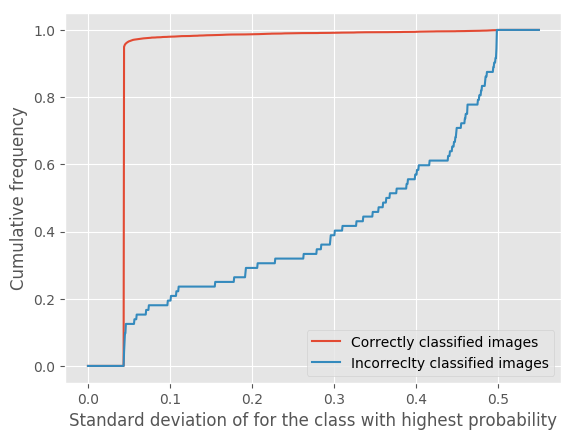
\includegraphics[scale=0.5]{mnist_cum_stds}
	\caption{Cumulative distribution of standard deviations for correctly and incorrectly classified test images. The standard deviation of the most likely class is taken for both correctly and incorrectly classified images.}
	\label{fig/mnist_cum_stds}
\end{figure}

\subsection{Noisy MNIST (n-MNIST)}
Next, I evaluate both the CNN and the Gaussian process on the n-MNIST dataset \cite{DBLP:journals/corr/BasuKGDMN15}. The dataset consists of the MNIST images, but modified in 3 different ways so as to make the classification task harder. The first set of images is created by adding white Guassian noise with a signal-to-noise ratio of 9.5 to the images. The second set of images is obtained by emulating a linear motion blur. The last set of images is the hardest to classify as it is created by reducing the contrast and also adding white Guassian noise to the original images. Figure \ref{fig/noisy_mnist_example} shows an example image taken from the 3 datasets.

\begin{figure}[h]
	\centering
	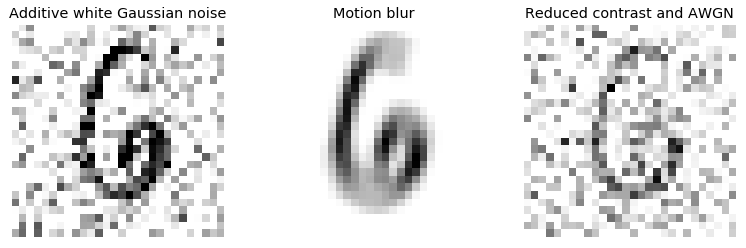
\includegraphics[scale=0.3]{noisy_mnist_example}
	\caption{Example digits from the noisy-MNIST dataset. From left to right: Additive white Guassian noise, Motion blur, and Reduced contrast with AWGN}
	\label{fig/noisy_mnist_example}
\end{figure}

The task of classifying examples whose underlying distribution is different from the underlying distribution of the training images is called \textbf{out-of-distribution} classification (CITE GAL DISSERTATION). The performance of the two models is shown in table \ref{table/noisy_mnist_acc}. Although the GP performs better on the NMIST test images, the CNN performs better on all 3 noisy datasets. This could be explained by the fact that the GP is a more complex model, and therefore is overfitting more on the NMIST data. Especially noticeable is the difference in performance for the reduced contrast dataset, where the CNN obtains an accuracy of $77.71\%$ compared to $70.13\%$ for the GP. As the 3\textsuperscript{rd} dataset is the least similar the original one, this higher discrepancy supports the claim that the GP is overfitting more on the MNIST dataset.

\begin{table}[h]
\centering	
{\renewcommand{\arraystretch}{1.4} %<- modify value to suit your needs
\begin{tabular}{ c | c c c}
\textbf{Model} & \multicolumn{3}{c}{\textbf{Accuracy}}\\
& AWGN & Motion blur & Reduced contrast\\
\hline
CNN & $94.35\%$ & $93.27\%$ & $77.71\%$ \\
GP & $93.34\%$  & $92.09\%$ & $70.13\%$ \\
\end{tabular}
}
\caption{MNIST test images accuracy for the CNN and the GP.}
\label{table/noisy_mnist_acc}
\end{table}

We can again inspect how uncertain the model is when classifying the noisy dataset, by plotting the cumulative distributions of the standard deviations of the most likely digit for the 3 datasets. Figure \ref{fig/noisy_mnist_cum_stds} shows the resulting plots, which indeed suggest that the uncertainty increases as the model is asked to classify images that are increasingly different images from those it was trained on. The uncertainty for the additive white Guassian noise (AWGN) images is higher than the uncertainty for the standard MNIST test set. This is shown by the fact that the cumulative distribution for the correctly classified images in the AWGN images is lower. Similarly, the cumulative distribution further decreases for the motion blur and reduced contrast images, with a lower classification accuracy corresponding to a higher uncertainty.

\begin{figure}[H]
	\centering
	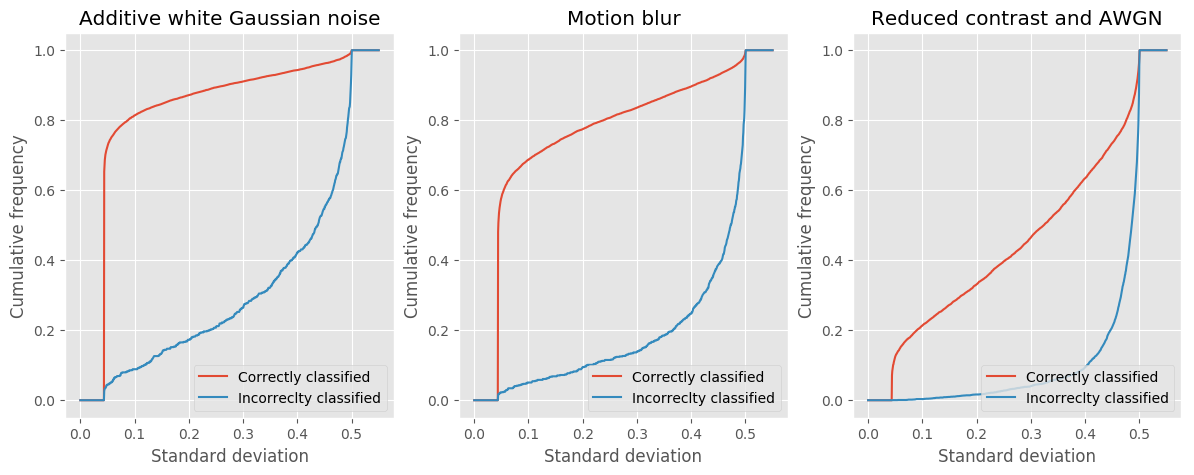
\includegraphics[scale=0.4]{noisy_mnist_cum_stds}
	\caption{Cumulative distribution of standard deviations for correctly and incorrectly classified test images. The standard deviation of the most likely class is taken for both correctly and incorrectly classified images.}
	\label{fig/noisy_mnist_cum_stds}
\end{figure}


\subsection{Classifying with a reject option}


\subsection{Uncertainty with additive white noise}
\begin{figure}[h]
	\centering
	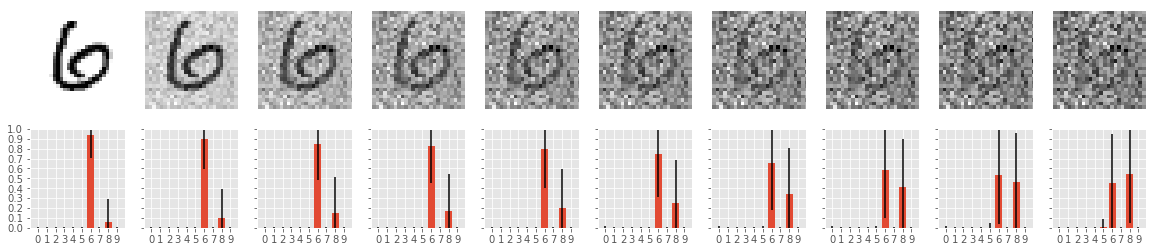
\includegraphics[width=1.0\textwidth]{awgn_predictions}
	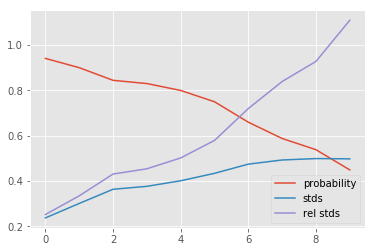
\includegraphics[scale=0.4]{awgn_predictions_stds}
	\caption{Cumulative distribution of standard deviations for correctly and incorrectly classified test images. The standard deviation of the most likely class is taken for both correctly and incorrectly classified images.}
	\label{fig/awgn_predictions}
\end{figure}

\subsection{Uncertainty with rotated images}
TODO: Use rotation of an image, e.g. Yarin Gal


\section{Discussion}
More quantitave evalution of the results.

Show examples of images that are missclassified.
\begin{figure}[h]
	\centering
	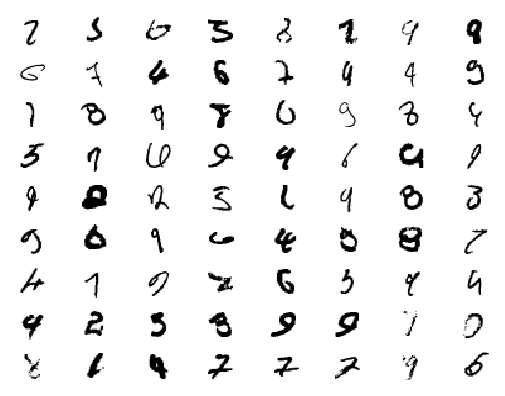
\includegraphics[scale=0.6]{incorrect_mnist}
	\caption{Test images misclassified images by the GP model.}
\end{figure}


Discuss definition of the metrics.

TODO: ADD VISUALLISATION of n-MNIST features
\subsection{CNN features visualisation}
\begin{figure}[h]
	\centering
	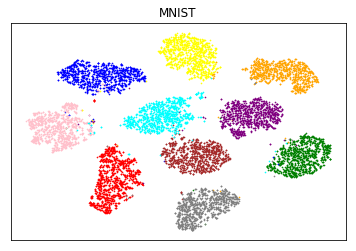
\includegraphics[scale=0.5]{embeddings_visualisation.png}
	\caption{Test point embedding using t-SNE}
\end{figure}

\small

\bibliography{bib}
\bibliographystyle{unsrt}


\end{document}
